\documentclass[tikz,border=2pt]{standalone}
\usepackage{amsmath}
\usetikzlibrary{arrows.meta}
\begin{document}
% Orthogonal projection onto a plane W: b = p + e with p = proj_W b in W and e perpendicular to W;
% for any other w in W the triangle b, p, w has a right angle at p, so ||b - w||^2 = ||e||^2 + ||p - w||^2.
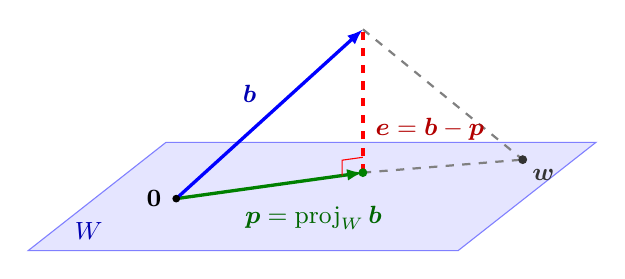
\begin{tikzpicture}[font=\small, >={Latex[length=2mm]}, x={(1.3cm,0cm)}, y={(0.7cm,0.55cm)}, z={(0cm,1.3cm)}]
  % the subspace W
  \fill[blue!10] (-0.8,-1.2,0) -- (3.4,-1.2,0) -- (3.4,1.3,0) -- (-0.8,1.3,0) -- cycle;
  \draw[blue!50] (-0.8,-1.2,0) -- (3.4,-1.2,0) -- (3.4,1.3,0) -- (-0.8,1.3,0) -- cycle;
  \node[blue!70!black] at (-0.45,-0.75,0) {$W$};
  % another point w of W and the right triangle b, p, w
  \draw[gray, thick, dashed] (1.5,0.6,1.4) -- (2.9,0.9,0);
  \draw[gray, thick, dashed] (1.5,0.6,0) -- (2.9,0.9,0);
  \fill[gray!40!black] (2.9,0.9,0) circle (1.6pt);
  \node[gray!40!black, anchor=north west] at (2.9,0.9,0) {$\boldsymbol{w}$};
  % projection, error and b
  \draw[->, green!50!black, very thick] (0,0,0) -- (1.5,0.6,0);
  \node[green!40!black, anchor=north west] at (0.55,0.05,0) {$\boldsymbol{p}=\operatorname{proj}_W\boldsymbol{b}$};
  \draw[red, very thick, dashed] (1.5,0.6,0) -- (1.5,0.6,1.4);
  \node[red!70!black, anchor=west] at (1.53,0.6,0.42) {$\boldsymbol{e}=\boldsymbol{b}-\boldsymbol{p}$};
  \draw[red] (1.5,0.6,0.15) -- (1.333,0.533,0.15) -- (1.333,0.533,0);
  \draw[->, blue, very thick] (0,0,0) -- (1.5,0.6,1.4);
  \node[blue!70!black, anchor=south east] at (0.72,0.29,0.72) {$\boldsymbol{b}$};
  \fill[green!50!black] (1.5,0.6,0) circle (1.6pt);
  \fill (0,0,0) circle (1.4pt);
  \node[anchor=east] at (-0.05,0,0) {$\boldsymbol{0}$};
\end{tikzpicture}
\end{document}
